\documentclass{beamer}
\DeclareFontShape{OT1}{cmss}{b}{n}{<->ssub * cmss/bx/n}{} 
\usetheme{default}
\usepackage{amsmath}
\usepackage{amsfonts}
\usepackage{mathbbol}
\usepackage{xcolor} % before tikz or tkz-euclide if necessary
\usepackage{tkz-euclide} % no need to load TikZ
\usepackage{multirow}
\usepackage{lmodern}
\usepackage{bm}

\titlegraphic{
\includegraphics[width=2cm]{../../Figures/UAMS_RGB.png}
}


\title{Statistical Machine Learning\\ Part 8\\ Random Forest}
\author{Horacio G\'omez-Acevedo\\ Department of Biomedical Informatics\\
University of Arkansas for Medical Sciences}
\begin{document}
	\begin{frame}[plain]
		\maketitle
	\end{frame}
	\begin{frame}{Bagging}
		
		We have seen that regression (or classification) trees are very useful but particularly unstable. That is, they suffer from high variance when presented with new data. 
		
		Fortunately, there is a general purpose procedures to reduce variance called {\it Bootstrap aggregation} or {\it bagging}. 
		
		{\bf Key Idea:} Given a set of $m$ independent (and identically distributed)  observations $X_1,\ldots, X_m$ each with variance $\sigma^2$, the variance of the mean $\overline{X}$ is given by 
		\begin{equation*}
			\hat{\sigma}^2(\overline{X})= \frac{1}{m} \sigma^2
		\end{equation*}
		{\bf Averaging a set of observations reduces variance}
		
	\end{frame}

\begin{frame}{Bagging (cont)}
	
	It seems reasonable that for a given model $Y=f(X)+\varepsilon$ to get an estimate response at the point $X=x$ by averaging $\hat{f}^1(x), \ldots, \hat{f}^B(x)$ using $B$ separate training sets, that is 
	\begin{equation*}
		\hat{f}_{\textrm{avg}}(x)= \frac{1}{B} \sum_{b=1}^B \hat{f}^b (x)
	\end{equation*}

where $\hat{f}^k$ is a tree regression estimate (without pruning) based on the observations $\{x_{k1},\ldots,x_{kB}\}$.

Since we don't have multiple training sets, then we exploit {\bf bootstrap!}.  More precisely, for a bootstrapped training set $b$, we obtain the estimate $\hat{f}^{*b}(x)$, and the corresponding {\bf bagging estimate}

	\begin{equation*}
	\hat{f}_{\textrm{bag}}(x)= \frac{1}{B} \sum_{b=1}^B \hat{f}^{*b} (x)
\end{equation*}

\end{frame}
	
	
	



\begin{frame}{Bagging for Regression Trees}
	
	There are few steps that we need to take for regression trees
	\begin{itemize}
		\item Construct $B$ regression trees using $B$ bootstrapped training sets (without pruning)
		\item Average the resulting predictions
	\end{itemize}
Keep in mind that each (bootstrapped) tree has low bias but high variance. The bagging procedure will reduce the variance at the expense of a "modest" increase in bias. 
\end{frame}

\begin{frame}{Bagging for Classification Trees}
	
	The steps are similar for classification trees
	\begin{itemize}
		\item Construct $B$ regression trees using $B$ bootstrapped training sets (without pruning)
		\item The prediction will be based on the majority vote. That is, the class most commonly occurring will be selected.
	\end{itemize}

\end{frame}

\begin{frame}{Out-of-Bag Observations}
	
	The main idea of the bootstrap is that from $m$ observations, we select a sample with replacement $m$ observations.
	
	What is the probability of {\bf not} selecting sample 1 ?
	
	The probability of picking sample different from 1 would be 
	$(1 - \frac{1}{m})$. Since we are repeating the experiment with replacement, the probability that a bootstrap sample does not contain sample 1 is 
	\begin{equation*}
		\left(1 - \frac{1}{m}\right) \cdot \left(1 - \frac{1}{m}\right) \cdots \left(1 - \frac{1}{m}\right) = \left(1 - \frac{1}{m}\right)^m
	\end{equation*}
	 A little bit of calculus shows that 
	 \begin{equation*}
	 \lim_{m\to\infty}\left(1-\frac{1}{m}\right)^m= \exp(-1) \approx 36.79\%
	 \end{equation*}
Thus, bootstrapping will not touch about 1/3 of the observations!
and those observations are referred to as {\bf Out-of-Bag (OOB)}.  
\end{frame}

\begin{frame}{OOB Error Estimation}
	We can exploit the OOB observations to estimate the test error in the bagging process without the need of cross-validation or even a split of the data in training and testing.
	
	Once we have obtained our $\hat{f}_{bag}(x)$, we can use the OOB observations (i.e., observations not used for the bagging estimation) to determine predictions. 
	
	More precisely, we obtain $\hat{f}_{\textrm{oob}}^i (x)$ based on the OOB observations $\{x_{i1},\ldots, x_{iK}\}$, where $K \approx B/3$ for $B$ big enough. 
		
		
	
	
	\begin{equation*}
		\hat{f}_{OOB}(x)= \frac{1}{K}\sum_{i=1}^{K} \hat{f}^{i}_{\textrm{oob}}(x)
	\end{equation*}
This procedure leads to the calculation of the test MSE that is a valid estimate since the response is derived from trees that were not involved in the bagged model.

A similar expression is valid for classification, but instead of the average we can use the majority vote and purity metrics instead of MSE or RSS. 
\end{frame}


\begin{frame}{Variable Importance Measures}
	
	We know that bagging improves the accuracy in our predictions, at the expense of making our models harder to interpret. 
	
	For bagging regression trees, we use the {\bf Variable Importance Measure (VIM)} that is defined as the total amount that the RSS is decreased due to splits over the given predictor, averaged over all $B$ trees.  The larger the VIM, the more "relevant" is that predictor.
	
	For bagging classification trees, we can define VIM as the total amount that the Gini index (or cross-entropy) is decreased by splits over a given predictor, averaged over all $B$ trees. 
\end{frame}

\begin{frame}{VIM example}
	The {\tt Heart} data set VIM plot with a mean decrease of GIni index and normalized VIM is shown below.
	 \begin{figure}[h]
		\centering
		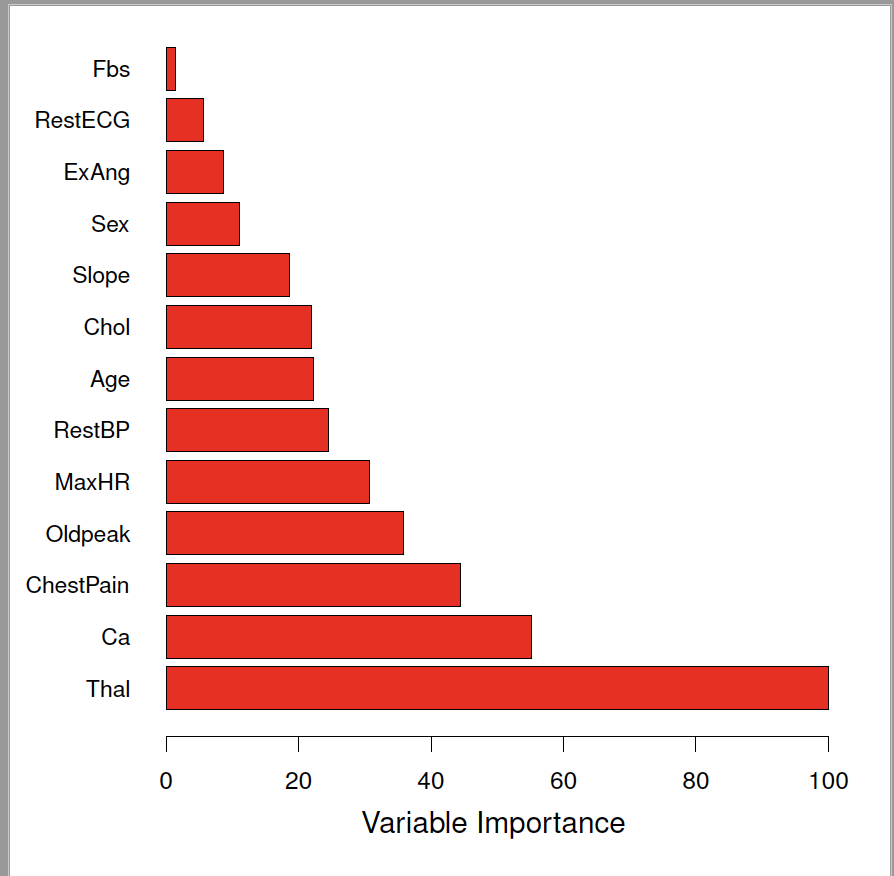
\includegraphics[scale=0.35]{../../Figures/fig_vim.png}
	\end{figure}
	
\end{frame}

\begin{frame}{Random Forest}
	It follows similar rationale as in bagging but with an interesting random twist.
	
	We build a number of decision trees on bootstrapped training samples. But when building these decision trees, each time a split in a tree is considered, a {\it random sample of $m$ predictors} is chosen as split candidates from the full set of $p$ predictors.  We normally set $m\approx \sqrt{p}$.
	
	What is the advantage of random forest over bagging?
	
	When we have a strong predictor, bagging trees will consider that predictor frequently, thus bagging trees will look alike. By having a random choice on the predictors, we may generate "different" trees that otherwise we would not have explored. This process is referred to as {\it decorrelating trees}. 

\end{frame}

\begin{frame}{Random Forest vs Bagging}
	The test errors from the {\tt Heart} data are depicted below
	 \begin{figure}[h]
		\centering
		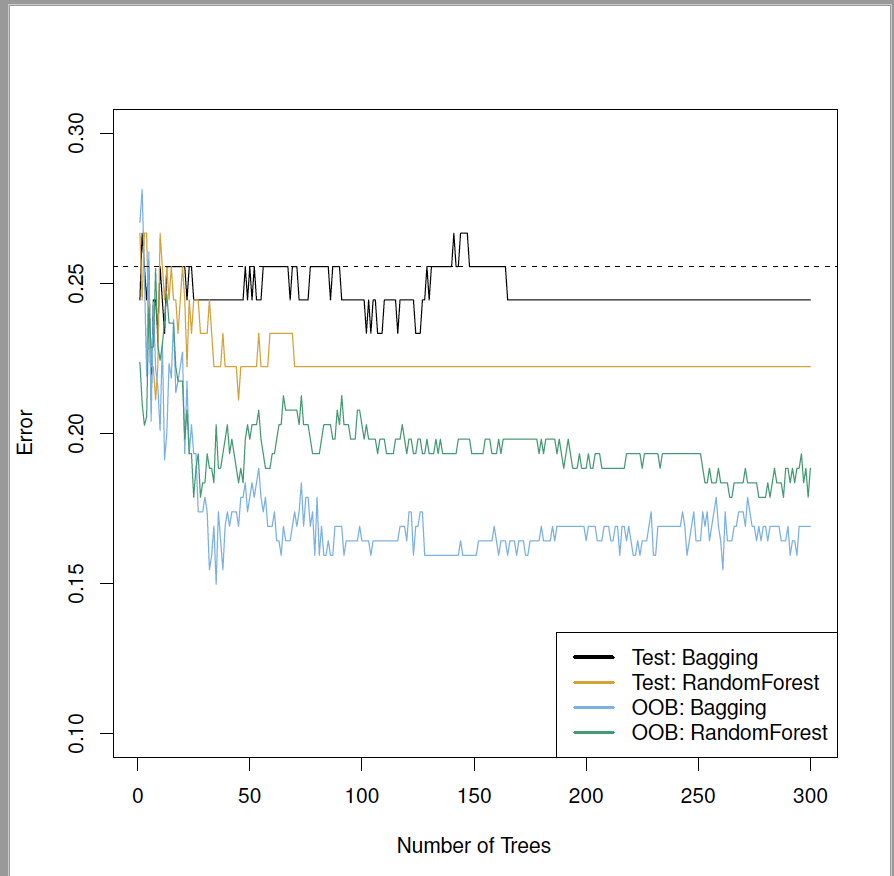
\includegraphics[scale=0.35]{../../Figures/fig_bagging.png}
	\end{figure}
\end{frame}

\begin{frame}{Boosting}
	
	{\bf Boosting} is another general methodology to improve the predictions from a decision tree. 
	In this case trees are grown sequentially as they gather information from previously generated trees. 
	
 Boosting does not require bootstrap sampling as each tree is fit on a modified version of the original data set.
 
 
	
\end{frame}

\begin{frame}{Boosting Algorithm}
	\begin{enumerate}
		\item Set $\hat{f}(x)=0$ and $r_i=y_i$ for all $i$ in the training set. 
		\item for $b=1,\ldots, B$ repeat:
		\begin{enumerate}
			\item Fit a tree $\hat{f}^b$ with $d$ splits to the training data $(X,r)$.
			\item Update $\hat{f}$ by adding in a shrunken version of the new tree:
			\begin{equation*}
				\hat{f}(x) \leftarrow \hat{f}(x)+ \lambda \hat{f}^b (x)
			\end{equation*}
		\item Update the residuals,
		\begin{equation*}
			r_i \leftarrow r_i - \lambda \hat{f}^b(x_i)
		\end{equation*}
		\end{enumerate}
	\item Output the boosted model
	\begin{equation}
		\hat{f}(x)=\sum_{b=1}^B \lambda \hat{f}^b(x)
	\end{equation}
	\end{enumerate}
\end{frame}

\begin{frame}{Boosting}
	Given a current model, we fit a decision tree to the residuals from the model rather than the outcome $Y$ as the response. And we add these residuals to a new decision tree and update again the residuals. 
	
	Boosting has the following tuning parameters:
	
	\begin{itemize}
		\item $B$ that represents the number of trees. Do not take very large values of $B$ as boosting tends to overfit. We can use cross-validation to determine a good candidate for $B$.
		\item The shrinkage parameter $\lambda$ controls the learning rate. 
		\item The number of splits $d$ controls the complexity of the boosted ensemble. Sometimes $d=1$ works well. 
	\end{itemize} \end{frame}


\begin{frame}{Boosting}
	Boosting and random forest comparison in a 15-class gene expression data set to predict cancer.
	 \begin{figure}[h]
		\centering
		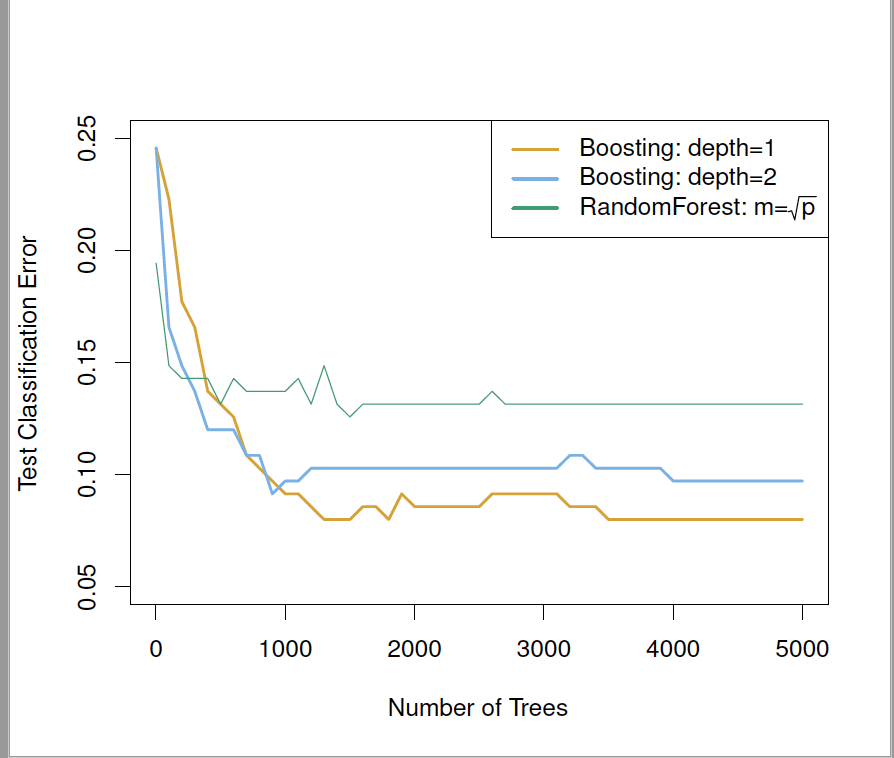
\includegraphics[scale=0.35]{../../Figures/fig_boosting.png}
	\end{figure}
	
\end{frame}

\begin{frame}{Final Thoughts}
	
 \begin{figure}[h]
	\centering
	\includegraphics[scale=0.05]{../../Figures/fig_comparison.png}
\end{figure}
\end{frame}

\begin{frame}{References}
	
	Materials and some of the pictures are from (1),(2), and (3).
	\begin{enumerate}
		\item Gareth James et al. {\it An Introduction to Statistical Learning with applications in R}. Springer (2015)
		\item Trevor Hastie et al. {\it The Elements of Statistical Learning } Springer (2001). 
		\item Aur\'elien G\'eron. {\it Hands-on Machine Learning with Scikit-Learn \& TensorFlow} O'Relly (2017)
		
	\end{enumerate}	
	
	I have used some of the graphs by hacking TiKz code from StakExchange, Inkscape for more aesthetic plots and other old tricks of \TeX
\end{frame}	


\end{document}